%%%%%%%%%%%%%%%%%%%%%%%%%%%%%%%%%%%%%%%%%%%%%%%%%%%%%%%%%%%%%%%%%%%%%%%%%%%%%%%%
%2345678901234567890123456789012345678901234567890123456789012345678901234567890
%        1         2         3         4         5         6         7         8

%\documentclass[letterpaper, 10 pt, conference]{ieeeconf}  % Comment this line out
                                                          % if you need a4paper
\documentclass[a4paper, 10pt, conference]{ieeeconf}      % Use this line for a4
                                                          % paper

\IEEEoverridecommandlockouts                              % This command is only
                                                          % needed if you want to
                                                          % use the \thanks command
\overrideIEEEmargins
% See the \addtolength command later in the file to balance the column lengths
% on the last page of the document



% The following packages can be found on http:\\www.ctan.org
%\usepackage{graphics} % for pdf, bitmapped graphics files
\usepackage{epsfig} % for postscript graphics files
%\usepackage{mathptmx} % assumes new font selection scheme installed
%\usepackage{times} % assumes new font selection scheme installed
%\usepackage{amsmath} % assumes amsmath package installed
%\usepackage{amssymb}  % assumes amsmath package installed

\title{\LARGE \bf
Autonomous Offensive Passing Systems for Robot Soccer
}

%\author{ \parbox{3 in}{\centering Huibert Kwakernaak*
%         \thanks{*Use the $\backslash$thanks command to put information here}\\
%         Faculty of Electrical Engineering, Mathematics and Computer Science\\
%         University of Twente\\
%         7500 AE Enschede, The Netherlands\\
%         {\tt\small h.kwakernaak@autsubmit.com}}
%         \hspace*{ 0.5 in}
%         \parbox{3 in}{ \centering Pradeep Misra**
%         \thanks{**The footnote marks may be inserted manually}\\
%        Department of Electrical Engineering \\
%         Wright State University\\
%         Dayton, OH 45435, USA\\
%         {\tt\small pmisra@cs.wright.edu}}
%}

\author{Alex Cunningham and Philip Rogers% <-this % stops a space
\thanks{This work was not supported by any organization}% <-this % stops a space
% \thanks{H. Kwakernaak is with Faculty of Electrical Engineering, Mathematics and Computer Science,
%         University of Twente, 7500 AE Enschede, The Netherlands
%         {\tt\small h.kwakernaak@autsubmit.com}}%
% \thanks{P. Misra is with the Department of Electrical Engineering, Wright State University,
%         Dayton, OH 45435, USA
%         {\tt\small pmisra@cs.wright.edu}}%
}


\begin{document}



\maketitle
\thispagestyle{empty}
\pagestyle{empty}


%%%%%%%%%%%%%%%%%%%%%%%%%%%%%%%%%%%%%%%%%%%%%%%%%%%%%%%%%%%%%%%%%%%%%%%%%%%%%%%%
\begin{abstract}

This project adds new passing capabilities to the GT Robojackets RoboCup Small Size League (SSL) robot team. The existing system supports moving, shooting, and can play the rules of soccer, but does not currently handle multirobot activity, such as passing, in a reliable manner. We extend the current system to implement a robust offensive passing system where the robots will acquire ball control and then make a coordinated series of passes until it can shoot on goal. We demonstrate a multi-stage planner that creates initial plans with an analytical planner and then performs nonlinear constrained optimization over the positions of robots to create an improved plan that mixed low-level controllers can execute.  

\end{abstract}


%%%%%%%%%%%%%%%%%%%%%%%%%%%%%%%%%%%%%%%%%%%%%%%%%%%%%%%%%%%%%%%%%%%%%%%%%%%%%%%%
\section{INTRODUCTION}
One of the larger robotics competitions in the world is the RoboCup competition, which seeks to build a robot soccer team that can beat a World Cup human team by the year 2050.  The subdivision in this project is the RoboCup Small Size League (SSL), in which a team plays 5-on-5 autonomous soccer.  What is notable about this league, is that due to the small size of the robots and omnidirectional drivetrain, the robots are extremely fast and agile, to a degree where humans are not capable of manually driving the robots nearly as well as autonomous control.  Due to this speed, SSL games provide an interesting domain for planning problems, as they are capable of playing a rather sophisticated game of soccer.  

The robot platform includes a team of robots controlled remotely via a centralized computer system, with an overhead vision system to determine the global position of the robots.  The centralization of the processing avoids many of the difficulties of using a true decentralized system, and as such more sophisticated gameplay occurs.  Our research builds on the existing system developed as a part of the Georgia Tech Robojackets RoboCup SSL team, currently ranked 2nd in the US, which includes a full fleet of robots and a simulator environment, in addition to the full robot control system.  

This project is an interesting planning challenge because of the speed of the robots and play that occurs in these games. Unlike the humanoid or four-legged-leagues, the Small Size League (SSL) robots are extremely fast in both motion and shooting, which makes the soccer games fast-paced, and reliant on effectively solving a number of sophisticated planning challenges simultaneously. To implement a basic passing system, the robots need to be able to move and plan in their space effectively, which is a non-trivial challenge because the robots have high enough acceleration to flip themselves over if they stop too quickly. Once a robot has a ball, the other robots need to position themselves to both receive an incoming pass and make another pass. While the number of robots is relatively small, such that a simple graph search can produce a series of passes to shoot on goal, handling the dynamic conditions of a high-speed game forces the planner to be more sophisticated. Because this is a soccer game, the primary 'obstacles' on the field are not just static or even dynamic obstacles, they are adversarial robots that will attempt to disrupt any plan execution that occurs. An effective planner in for these challenges must simultaneously manage basic motion planning for the robots, model passing sufficiently well to pass between the robots, find and replan optimal positions for robots. The additional constraint on the system is the uncertainty of the measurement, as there is noise in the robot position measurements, and especially the ball, which will disappear off of the global vision system if it moves too fast - a scenario that occurs almost every time a shot is made. 

\section{Related Work}

% this is put here to force it onto page 2 (at the end of related work)
% this is referenced in our methods section though.
\begin{figure*}[ht!]
\begin{center}
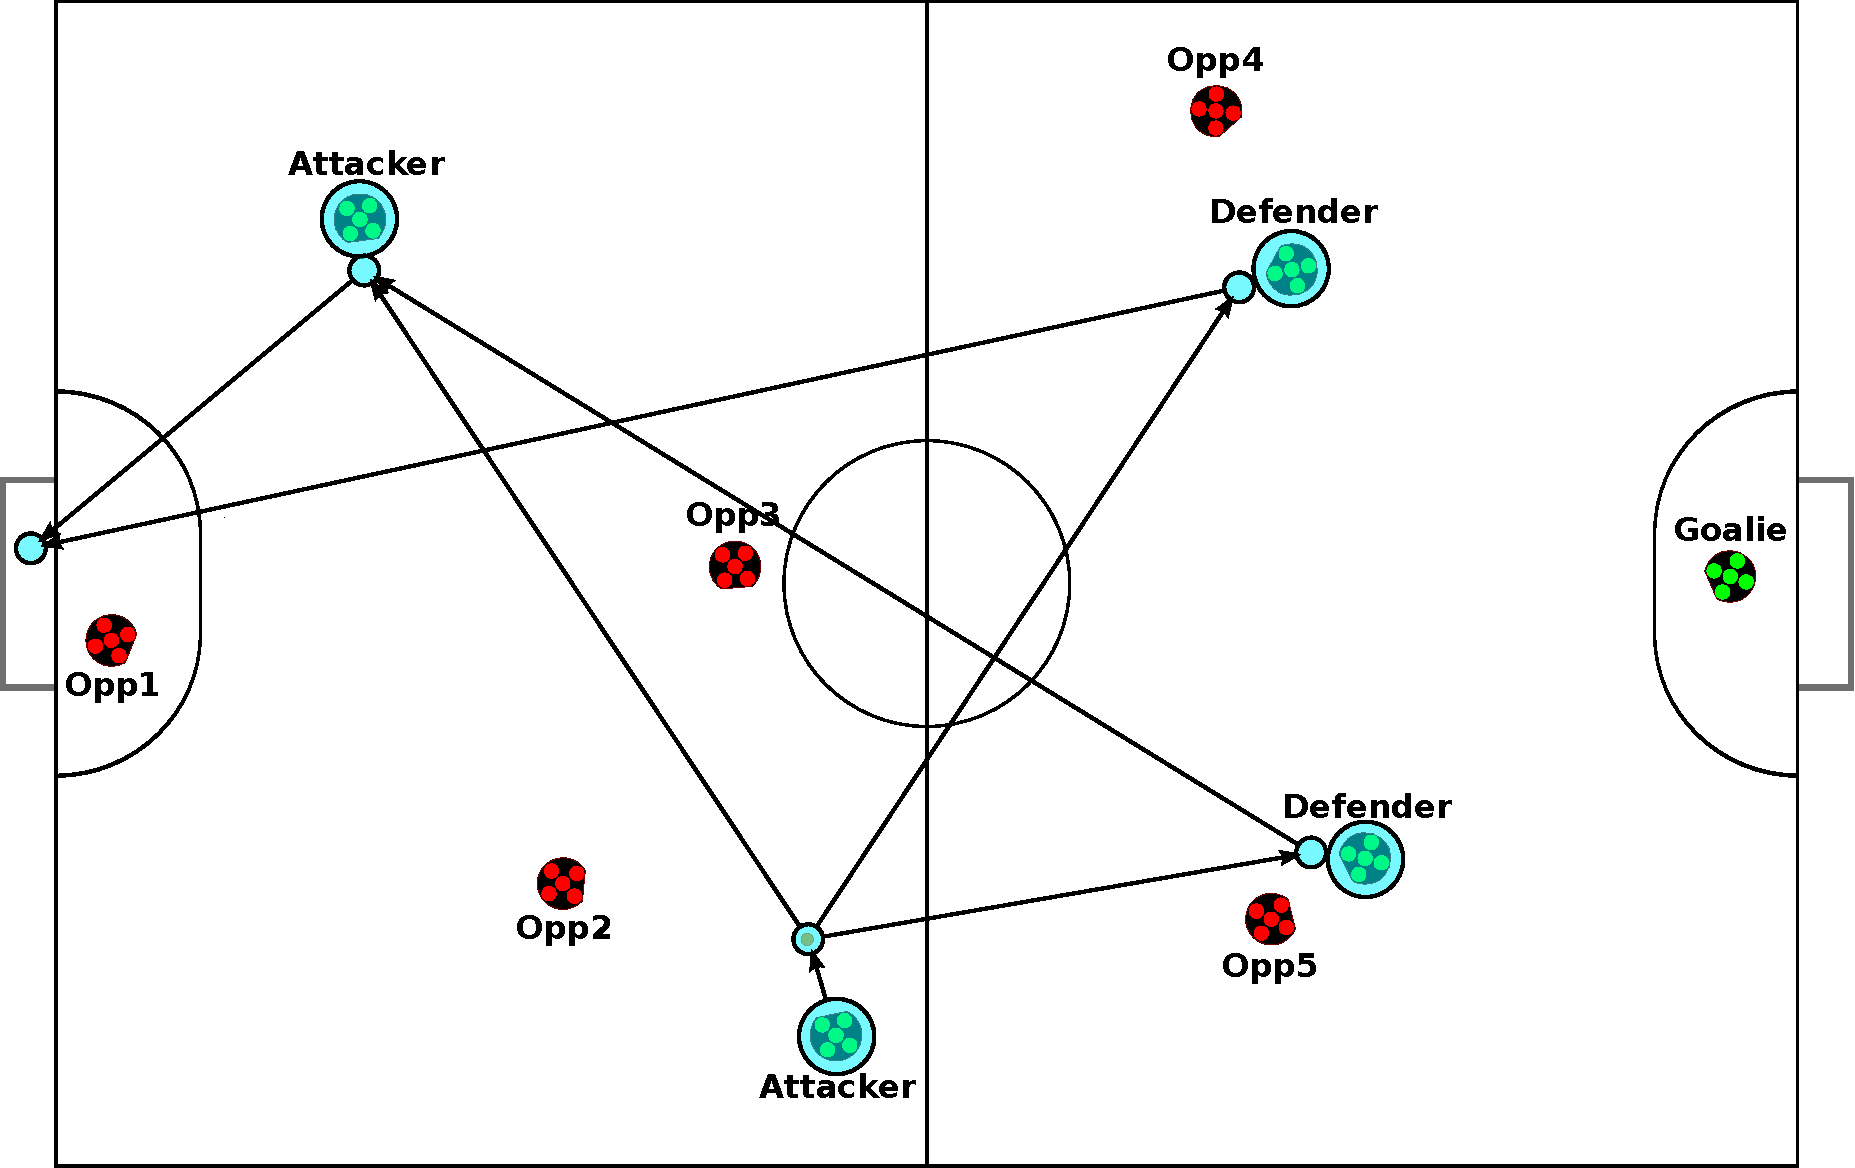
\includegraphics[totalheight=1.0in]{plan2_resized}
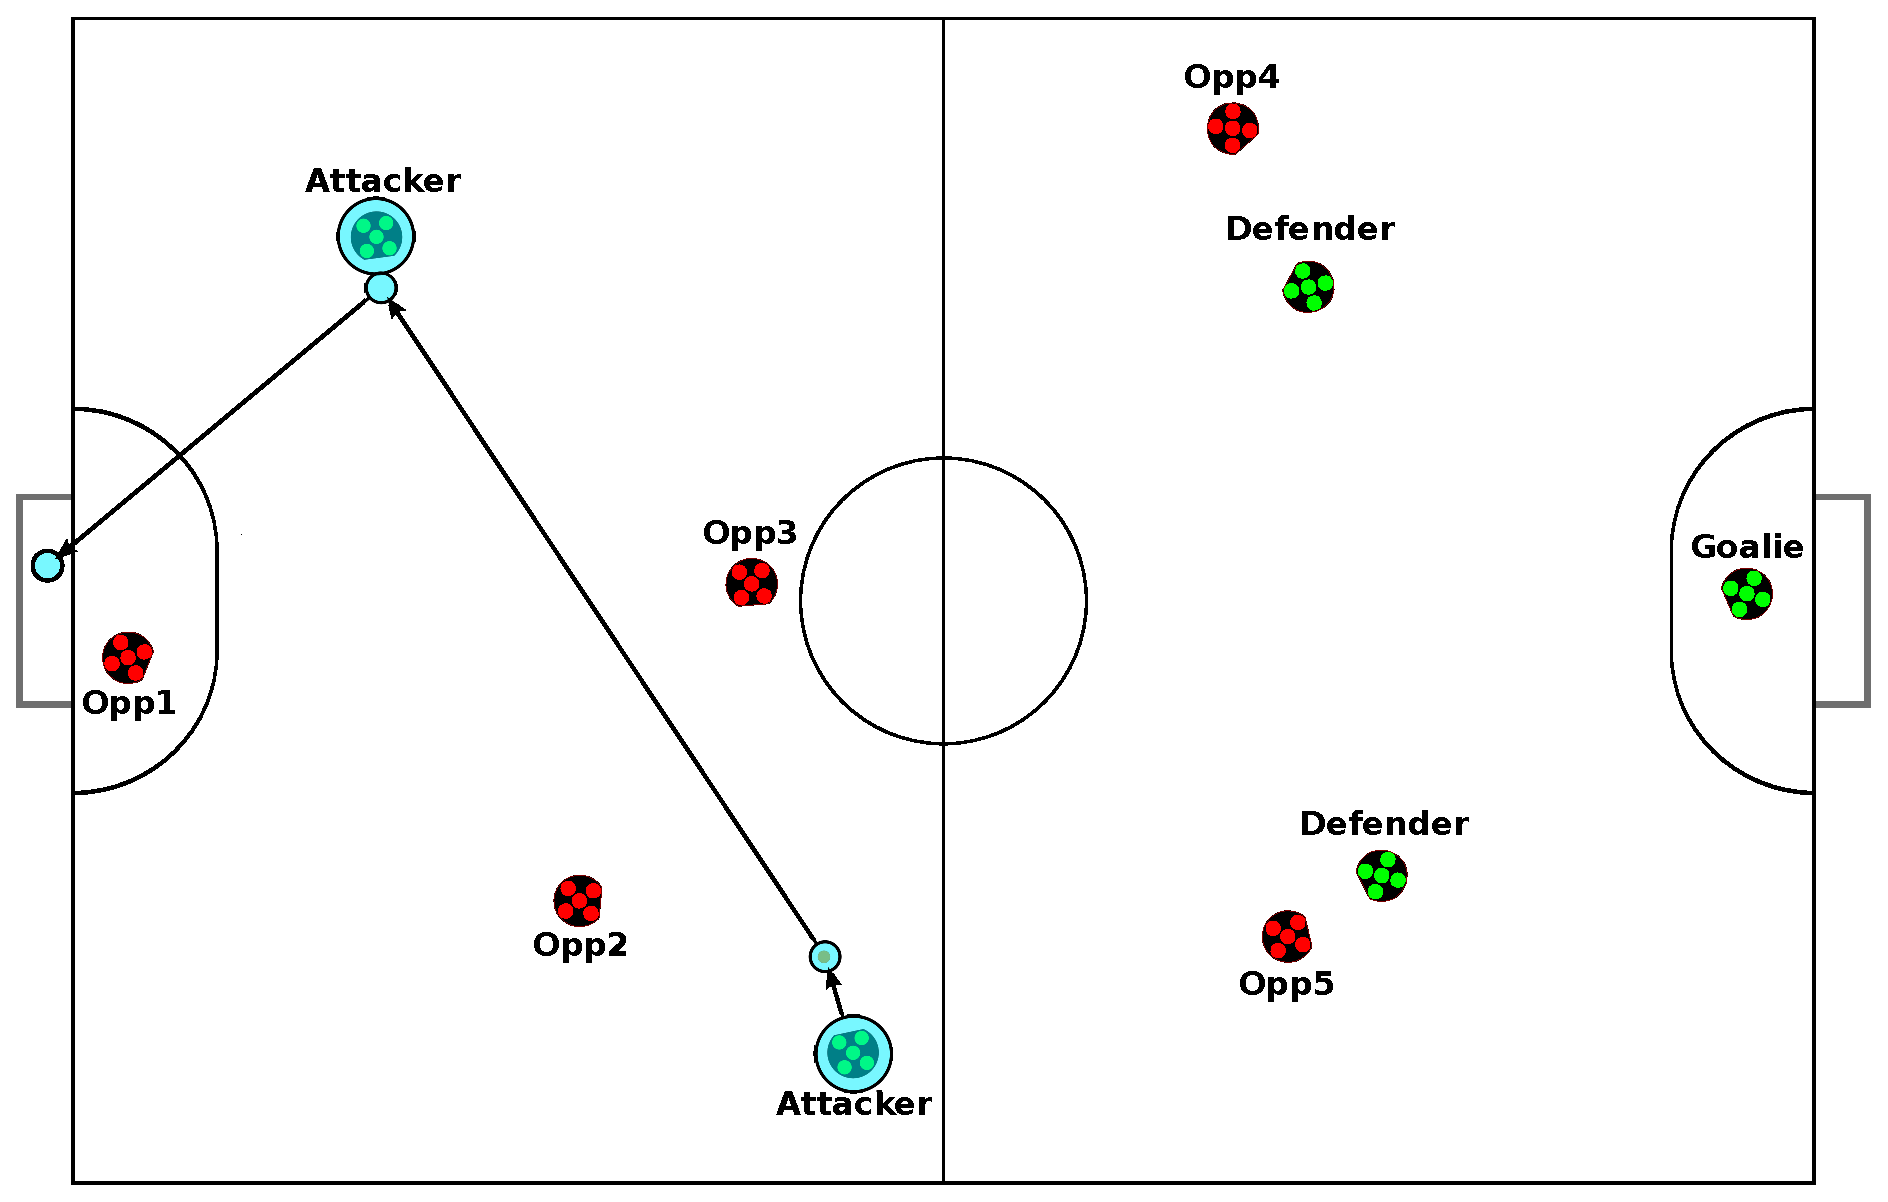
\includegraphics[totalheight=1.0in]{plan3_resized}
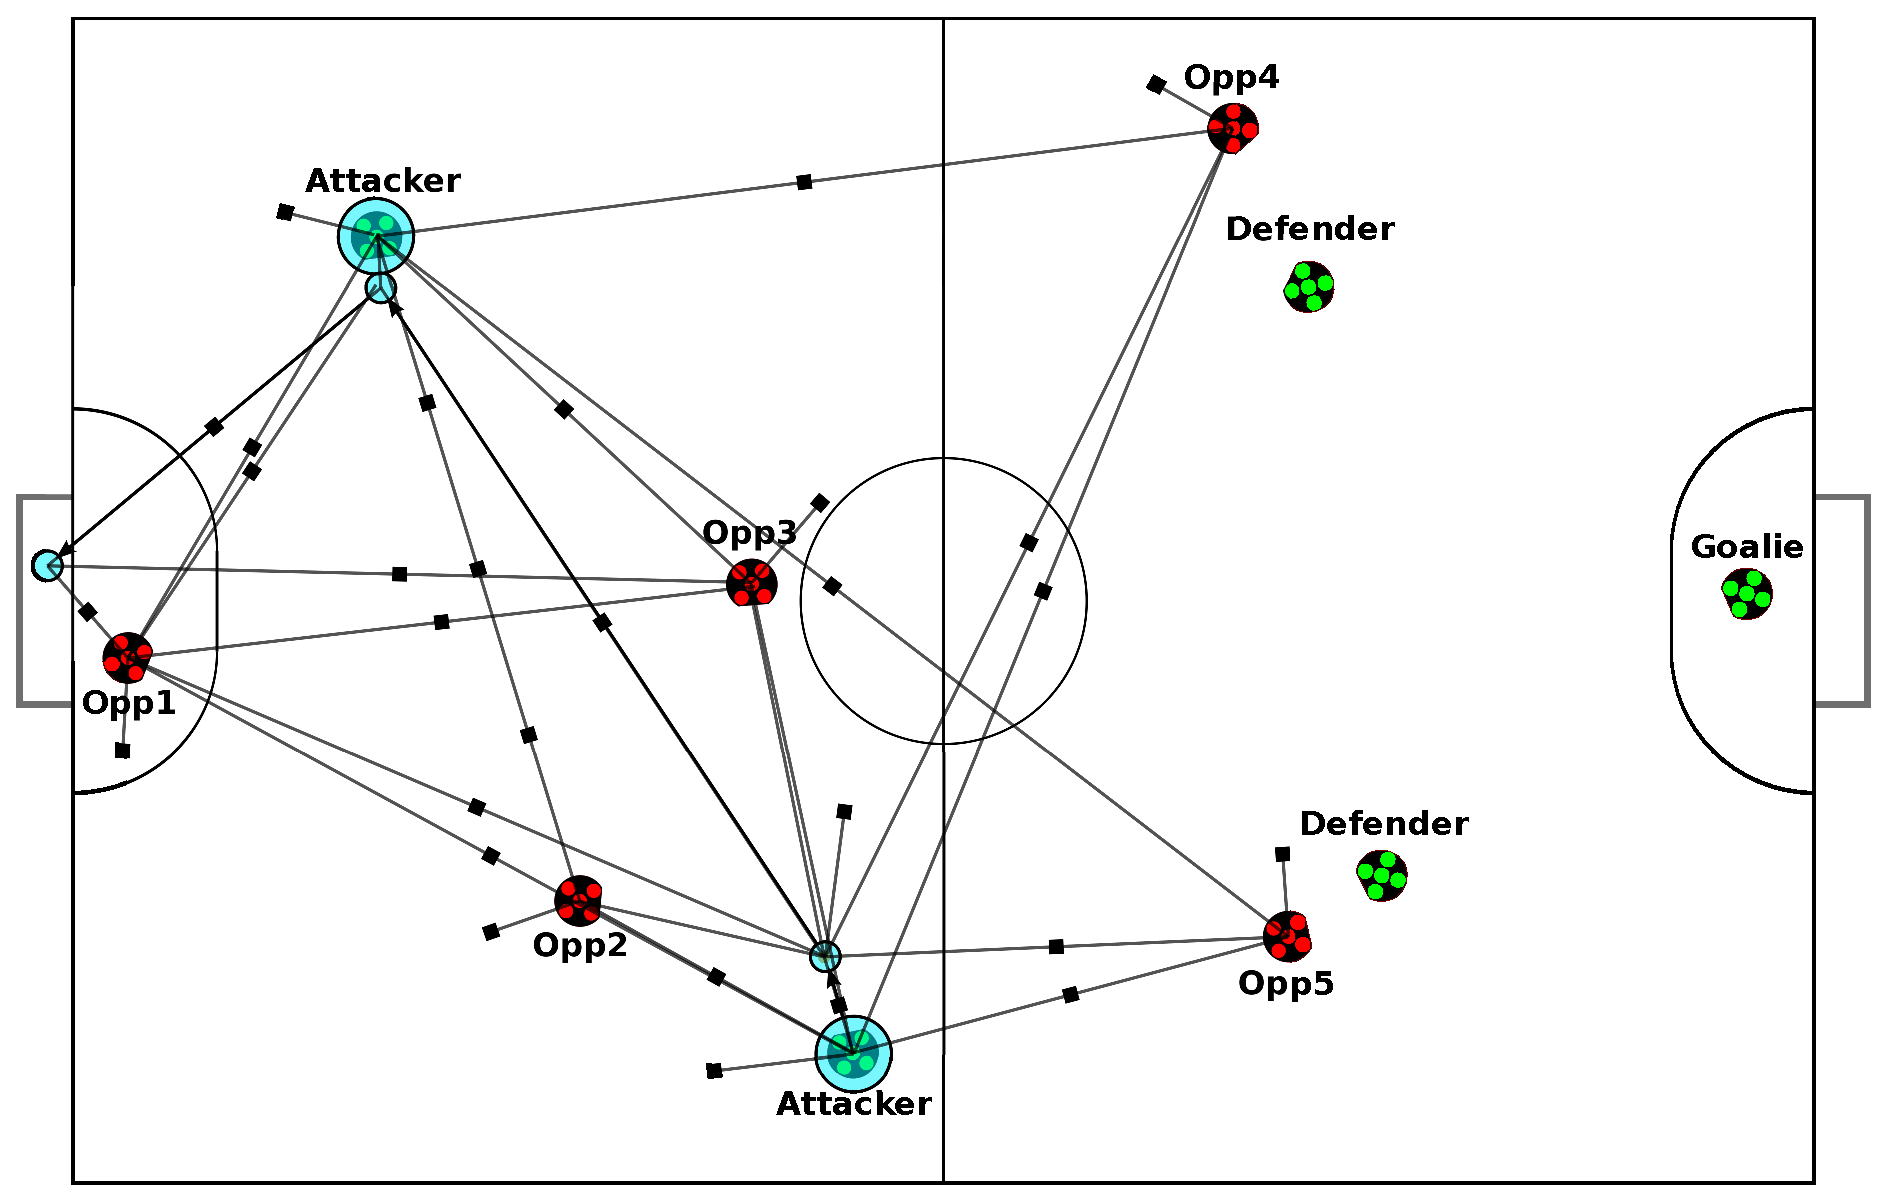
\includegraphics[totalheight=1.0in]{plan5_resized}
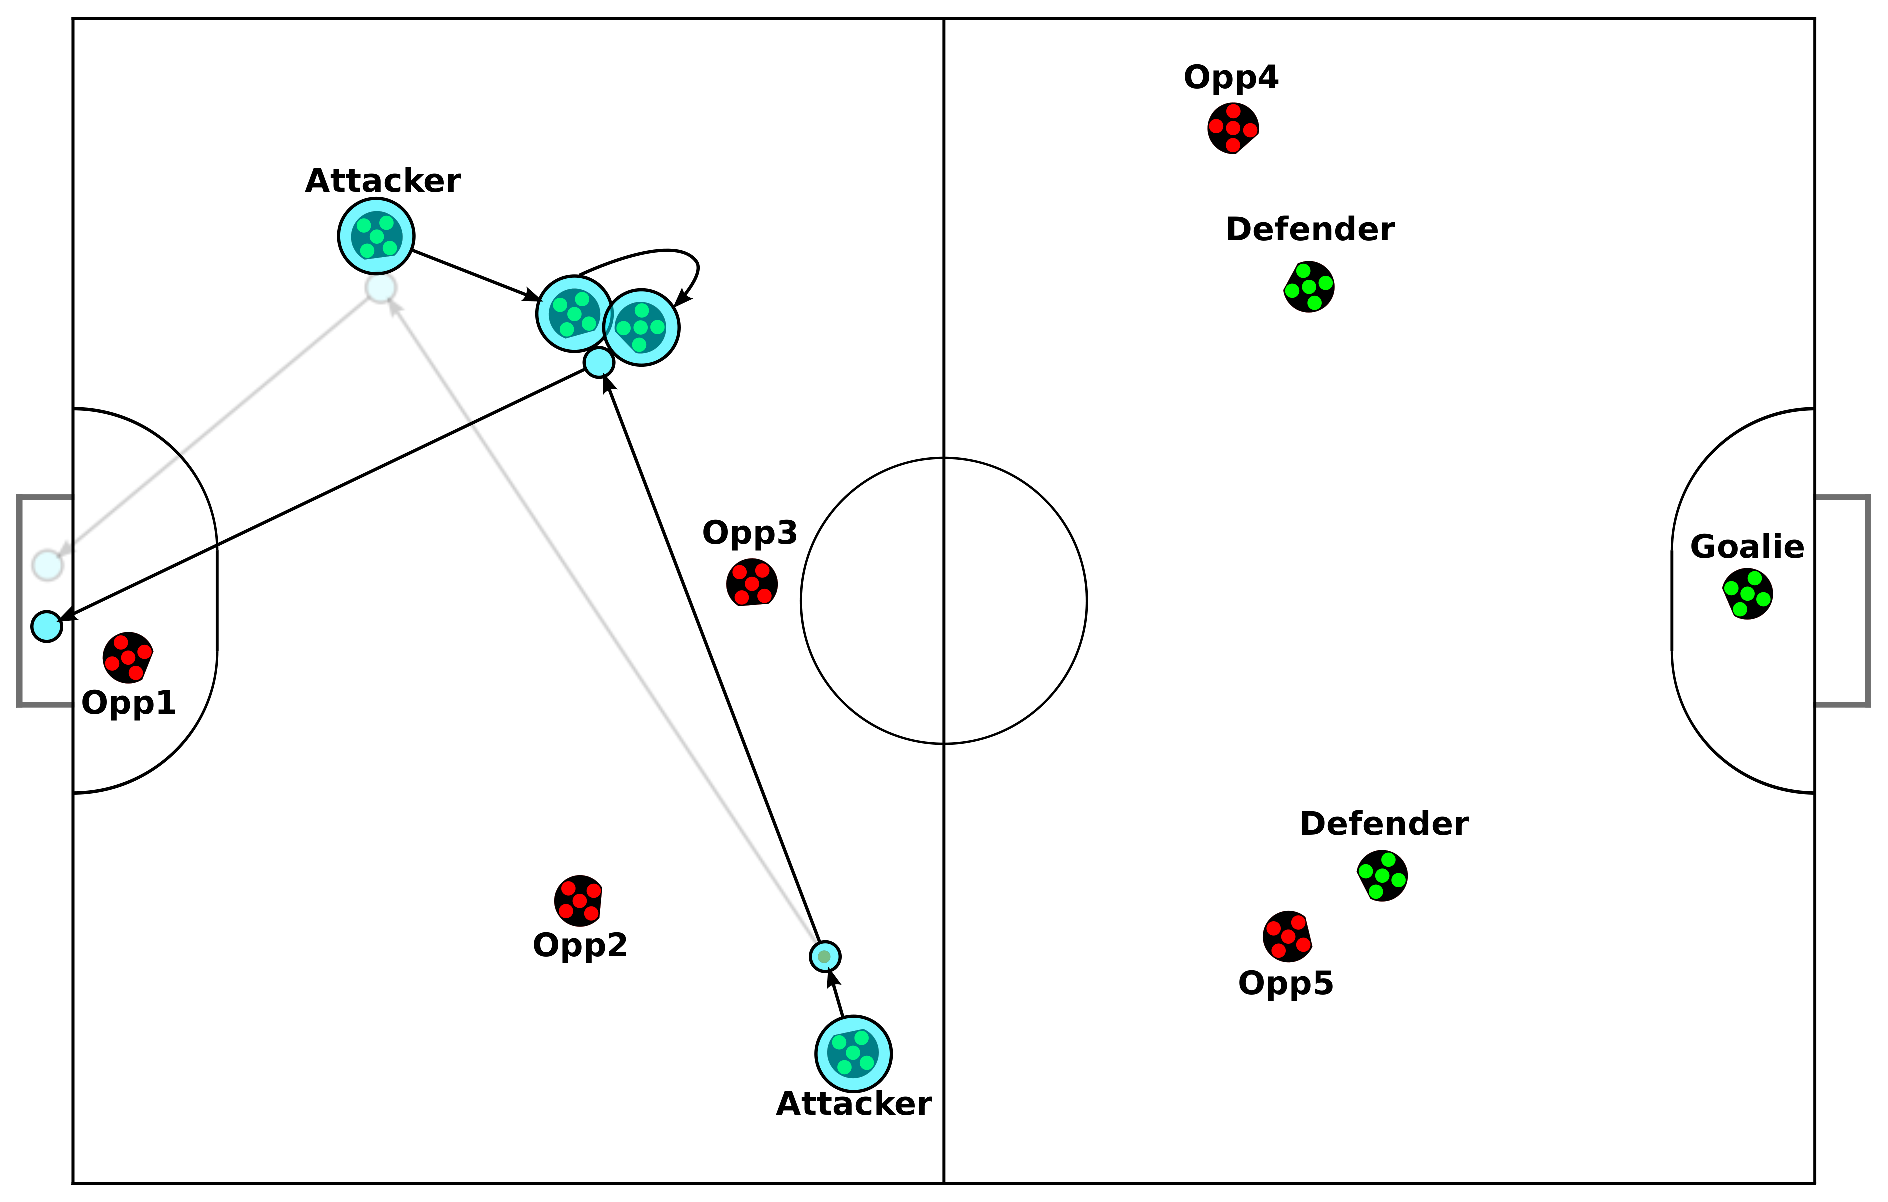
\includegraphics[totalheight=1.0in]{plan4_resized}
\end{center}
\caption{Methods used: Left-to-right: (1.) Analytic planner result (2.) Plan evaluation and selection of feasible subset. (3.) Optimization of feasible subset of plans. (4.) Optimized result which is executed.}
\end{figure*}

\subsection{ROBOTIC SOCCER}

The Skills, Tactics and Plays (STP) framework is the primary technique used by top Robocup teams \cite{bruce2003multi}. STP is a hierarchical approach consisting of high-level ``plays'', mid-level ``tactics'', and low-level ``skills'' which supports global planning and is able to make use of teamplay at both the Plays and the Tactics levels \cite{browning2005stp}. In a passing scenario, STP could use an offense play, a passing tactic and a receiving tactic, and skills such as drive, turn or shoot. To achieve computationally fast, robust, and competitive passing, the CMDragons team has an evaluation technique which, given that a pass will occur, selects a near-optimal position for the receiving robot to achieve a clear path for the ball. CMDragons uses several pre-defined passing tactics such as one-touch pass-and-shoot and pass-receive-turn-shoot, which selected for at the play level.

The current top Robocup SSL team, Skuba, use a slight variation on the STP framework \cite{skubaETD}. Their top-level strategy module selects from a number of plays. Each play uses ``Positions'', such as Aggressor and Defender, that are assigned to individual robots. Passing is implemented by using a a special position, called "SpecialOp", which assists a regular position and accepts passes.

By not considering the low-level details of a plan at the plays and tactics level, STP can fail to optimally use the robots' potentials or fail to anticipate obstacles or constraints. This was recognized Zickler and Veloso, who have combined the skills and tactics of the STP into a Kinodynamic planner \cite{zickler2008playing}. This approach has produced impressive results in simulation, such as bouncing the ball off of other players, though it has not been used on real real-time robots.

\subsection{OPTIMIZATION}

There are a variety of means of approaching optimization in the context of high-dimensional systems, and this paper will focus on the relationship between optimizing robot trajectories in an optimal controls sense with recovering robot trajectories from measurements taken on the environment.  The Simultaneous Localization and Mapping (SLAM) problem is a canonical problem in the field, where an optimization algorithm must find the most likely position of a robot in an environment based on a series of measurements of the environment.  Much of the work in the field has focused on approaching this problem using Kalman or particle filters  \cite{Thrun05book, Thrun04ijrr, Dellaert03tutorial} to represent the state of the system, however we will focus on solutions that provide the entire trajectory of the robot, otherwise known as the complete SLAM problem.  

The basic Smoothing and Mapping (SAM) approach\cite{Dellaert05tr} to the problem uses the Information Matrix to describe the relationships between variables, which can be used as an exact dual to the covariance matrix used in Kalman filters, but the key in the SAM approach is that this information matrix does not need to be kept in full form, rather, we can store the square root of the information matrix, which remains sparse during the course of optimization, a feature that we can exploit to perform much more efficient optimization.  The resulting operation used in solving SLAM problems becomes a matter of developing fast, multi-variable optimization algorithms, and there has been much work in this area to improve the underlying optimization techniques, particuarly from graph theory\cite{Triggs99, Bertele72jmaa, Bertele72book}.  In particular, there are methods for incremental SAM\cite{Dellaert06ijrr}, which are especially useful when approaching the development of real-time systems.

\section{METHODS}
In order to perform robust, efficient passing, we have decided on a particular structure for the offense play. The basic concept is that if there is a shot available or a sequence of passes to a shot (henceforth known as a "shooting solution"), then the system will construct the sequence of paths for robots and kicks, run a nonlinear optimization technique to improve the path and ensure viability, and then execute it.

This plan came out of two particular observations:

\begin{itemize}
 \item This bypasses the existing RRT-based planner, which is too unpredictable in timing for highly coordinated actions. We have no particularly good way of telling when a robot will reach a location when using RRTs.
 \item Because of the particular scenario of robot soccer, we know there are a small number of obstacles on the field, and there are only a small number of possible paths between them. With an optimization algorithm, we can take a simple path and improve it to make it faster.
\end{itemize}

The resulting system structure for the offensive passing algorithm has the following structure:
\begin{enumerate}
 \item \textit{Analytic Planner} Given the positions of all the robots and the ball, it is possible to determine if there is a shot solution available with a simple weighted graph search. This can be a simple heuristic for shot viability, or a more sophisticated system as necessary.
 \item \textit{Plan Evaluation} We take a set of plans and sort by quality on a number of metrics, so that a good initial estimate can be created.
 \item \textit{Optimization} With an initial estimate of a plan, the optimization engine will be able to create a graphical model of the plan and optimize for an optimal sequence of actions. The particular optimization engine is a nonlinear constrained optimization algorithm primarily designed for Simultaneous Localization and Mapping, but we will exploit the duality between this planning problem (create an optimal path from constraints) and SLAM (recover a previously traveled path given measurements).
 \item \textit{Execution} Given a viable plan a variety of motion planning and behavioral approaches can be used to to execute the actions that have been parameterized by plan generation and optimized.  
\end{enumerate}

The optimization algorithm comes from the gtsam library\cite{Dellaert05rss} developed in the RIM center with Frank Dellaert, and is derived from Sequential Quadratic Programming. This algorithm is robust to both nonlinear systems and constraints, and has been reformulated to work in a graphical model environment, which allows for an intuitive construction of stochastic switched hybrid systems.

\subsection{ANALYTIC PLANNING}
The analytic planner creates an initial structure of nodes representing robots, with links between them corresponding to the ball movement. This initial graph structure contains all possible combinations of passes with 1, 2, or 3 robots. Additional pass-lengths (such as 4-robot passes) are not considered due to the high probability of errors during passing. Using this high-level graph structure, we construct a cost function for pass solutions that penalizes passes that are too long or that are clearly blocked by either an opponent or another teammate. Special care is taken to not penalize solutions that have a possibility of being good passes at future levels of the planner. Using this cost function, we sort the possible passes and select a subset of the best passes to send to the optimization step.
The cost function used resembles the evaluation step in the STP planner, though it differs because our pass structure is created before any robot has the ball, and includes all possible passes, allowing us to optimize the passer and the receivers, as well as the ball path.

\subsection{OPTIMIZATION}
Once a plan has been selected for further evaluation, we use a constrained nonlinear optimization approach to find an improved solution.  A key observation in the development of the optimization technique is the dual nature between optimizing a robot control system and SAM.  In the SAM problem, the basic goal is to recover a robot trajectory based on a set of constraints from the robot's sensor systems and motion models after the robot has moved through the environment.  In the controls case, the goal is to determine an optimal trajectory based on a set of constraints, such as those on robot motion or obstacle avoidance.  In both cases, the goal is to recover a robot trajectory from a series of constraints, and they primarily differ in what sort of constraints are applied.  Rather than using the formulation of optimal control, we will use a graphical model approach to assemble a full cost function over the environment.  

There are two steps to effective optimization of a soccer plan:
\begin{itemize}
 \item \textit{Factor Graph Construction}: we assemble a cost function to optimize using a piecewise factor graph approach usually used in SAM solutions.  This allows development by means of combining a large number of constraint functions that individually relate only a small number of variables.
\item \textit{Nonlinear Optimization}: after the general cost function is assembled, we use Sequential Quadratic Programming (SQP) to reduce the a system with an arbitrary smooth nonlinear cost function and constraint set to a quadratic programming problem suitable for solving via Multi-frontal QR factorization.  
 \end{itemize}

The formulation of actual factors in this approach, as it derives from the need to define an error function in SAM, has the form of a function $h(x)$ dependent on the state of the system and a measurement $z$, where in the SAM case, the $h(x)$ is the generative measurement model and the $z$ is the actual value of the system, but in our system, $h(x)$ describes the current state with relation to a cost function, and $z$ is the optimal value.  Expressed in general form, these factors combine as in (\ref{factors}) to form a nonlinear least squares problem, where $x$ forms the set of state variables, $z_{k}$ is the optimal value for the constraint, and $R_{k}$ is a weighting matrix on the cost function.

\begin{equation} \label{factors}
 argmin(\frac{1}{2}\sum_{k}\left\Vert h_{k}(x_{k})-z_{k}\right\Vert _{R_{k}}^{2})
\end{equation} 

With this error-function approach, especially as it allows us to place relationships between variables in the system, we can build the cost function to define an optimal solution.  One of the basic cases where these cost functions can be assembled is to optimize for shorter passes between robots, as well as smaller robot movements, which can be expressed by using an optimal distance where $z=0$, and $h(x,y)=\left\Vert x-y \right\Vert$.  By connecting all of nodes with constraints such as these, we can simultaneously optimize the movement of robots and passes to find a series of movements and passes that minimizes all of the distances.  In this unconstrained optimization case, we can approach the actual optimization using nonlinear unconstrained optimization techniques such as Levenberg-Marquardt or Gauss-Newton. Because of the least-squares formulation of a quadratic cost function, we can approximate the Hessian of the overall cost function using only the Jacobian of $h(x)$.  The factor can be approximated through a linearization of the measurement function, which produces the Quadratic Programming problem shown in (\ref{eq:full_linear_factor}).  

\begin{equation} \label{eq:full_linear_factor}
argmin(\frac{1}{2}\sum_{k}\left\Vert H_{x_{k}}x+h(x_{k_{0}})-z\right\Vert _{R_{k}}^{2})
\end{equation}

Some other cases where factors define a means to improve a plan:
\begin{itemize}
 \item Maximizing the distance of pass trajectories from other robots to prevent pass interception.
 \item Maximizing the distance between robot paths and opponent robots to avoid collisions and improve movement speed.
 \item Minimizing the angle between the facing of a robot upon receiving a pass and making the next pass so as to minimize the time necessary aiming.  
\end{itemize}


While this works for basic scenarios, such as making the robots move and pass the smallest possible distance, we also need to express hard constraints on the motion nad passing of robots, such as staying on the field and not driving through other robots.  These constraints are not just cost functions to be minimized, but rather requirements that must be met for any solution to be feasible.  We can extend the previous expression to allow the incorporation of these hard constraints by redefining the optimization problem as a Lagrangian optimization problem, as in (\ref{constraints}).  

\begin{equation} \label{constraints}
 argmin(\frac{1}{2}\sum_{k}\left\Vert h_{k}(x_{k})-z_{k}\right\Vert _{R_{k}}^{2}-\lambda g(x))
\end{equation} 

We can express the constraints in the form of $g(x)$, where $g(x)$ defines a vector-valued function where the constraints are considered fulfilled if $g(x)\leq 0$, which allows both equality constraints, such as ensuring passes arrive at the same time and location as the robot receiving the pass, or inequality constraints, such as maintaining bounds on the positions, velocities and acceleration of the robots to keep them on the field and driving with viable commands.  The addition of these constraints requires a more sophisticated solution method, and in our case, we use Sequential Quadratic Programming (SQP) to reduce the full nonlinear constrained problem into a series of quadratic programming subproblems with linear constraints, which can then be solved with a mixture of direct elimination of the constrained variables, and unconstrained optimization on the remaining variables\cite{Fletcher87book}. 

To demonstrate the optimization in a simple environment, we reduced the optimization problem to finding new positions for each of the robots such that we minimize the distance of travel for both passes and robot movement.  We approximated robot motion to include only an initial and final state to allow for straight-line paths between points.  Due to this approximation, we more tightly constrained the distance the robots could move to prevent the need for more sophisticated obstacle avoidance techniques.  The optimization routine takes as input a set of robot positions in a passing sequence and provides a new set of robot positions that result in better passes.  

The factors and constraints used are as follows:
\begin{itemize}
 \item \textit{factor} Path shortening on robot movement
 \item \textit{factor} Path shortening on pass and shot lengths
 \item \textit{constraint} Robot initial positions are fixed to the real initial positions
 \item \textit{constraint} Robot positions must remain on the field to be viable
\end{itemize}

Even with this small set of factors, we can provide an expressive means to optimize robot control, and with additional factors we could find even better final pass sequences.  

\subsection{CONTROL}
In order translate the plans to robots in the actual system, we have a number of low-level controllers that execute commands. We can switch between various control approaches for particular applications, which can be necessary to avoid using suboptimal methods.  There are several means of issuing commands to the robots to execute movements across the field:
\begin{itemize}
 \item \textit{RRT Planning} For situations when we need a robot to move around other robots, we can use a simple RRT-based system to find a path.  This does, however, have the problem that the resulting path is unpredictable, so it cannot be used well with optimization-based approaches
 \item \textit{Direct Path Commands} We can instruct a robot to execute a specific path, which allows for more control by the higher-level modules in the system.  
 \end{itemize}

The low-level path execution uses a controller that drives the robots to their destinations as fast as possible with the ideal trapezoidal velocity profile.  Upon starting movement, the robot begins at maximum acceleration until it reaches maximum velocity, maintains the maximum velocity while following the path, and then slows at its maximum deceleration rate to stop at its goal.  The bounds used in this model derive from empirical tests of robot performance.  

While we do have direct control over the robots, there are still a number of areas of uncertainty in the robot commands, which limits the degree to which planning can look ahead into the future:
\begin{itemize}
 \item The control system currently only uses the vision system to provide robot positions, rather than direct wheel velocities, which makes the robots less responsive to commands.
 \item The ball position reported by the overhead camera has uncertainty in the positioning of the ball, especially when it is moving at high speeds, which can result in the vision system losing the ball.
 \item Kicking does not come in the form of a instananeous ``kick'' command, but rather a ``kick when ready'' because the ball must be exactly in front of the kicker bar on the robot.  This makes timing the kicks themselves more difficult.  
\end{itemize}

\section{EXPERIMENTS}
We tested the system using the simulated environment with the GT RoboCup software, which allows for an identical interface between the simulated environment and the real robots.

\begin{figure}[ht!]
\begin{center}
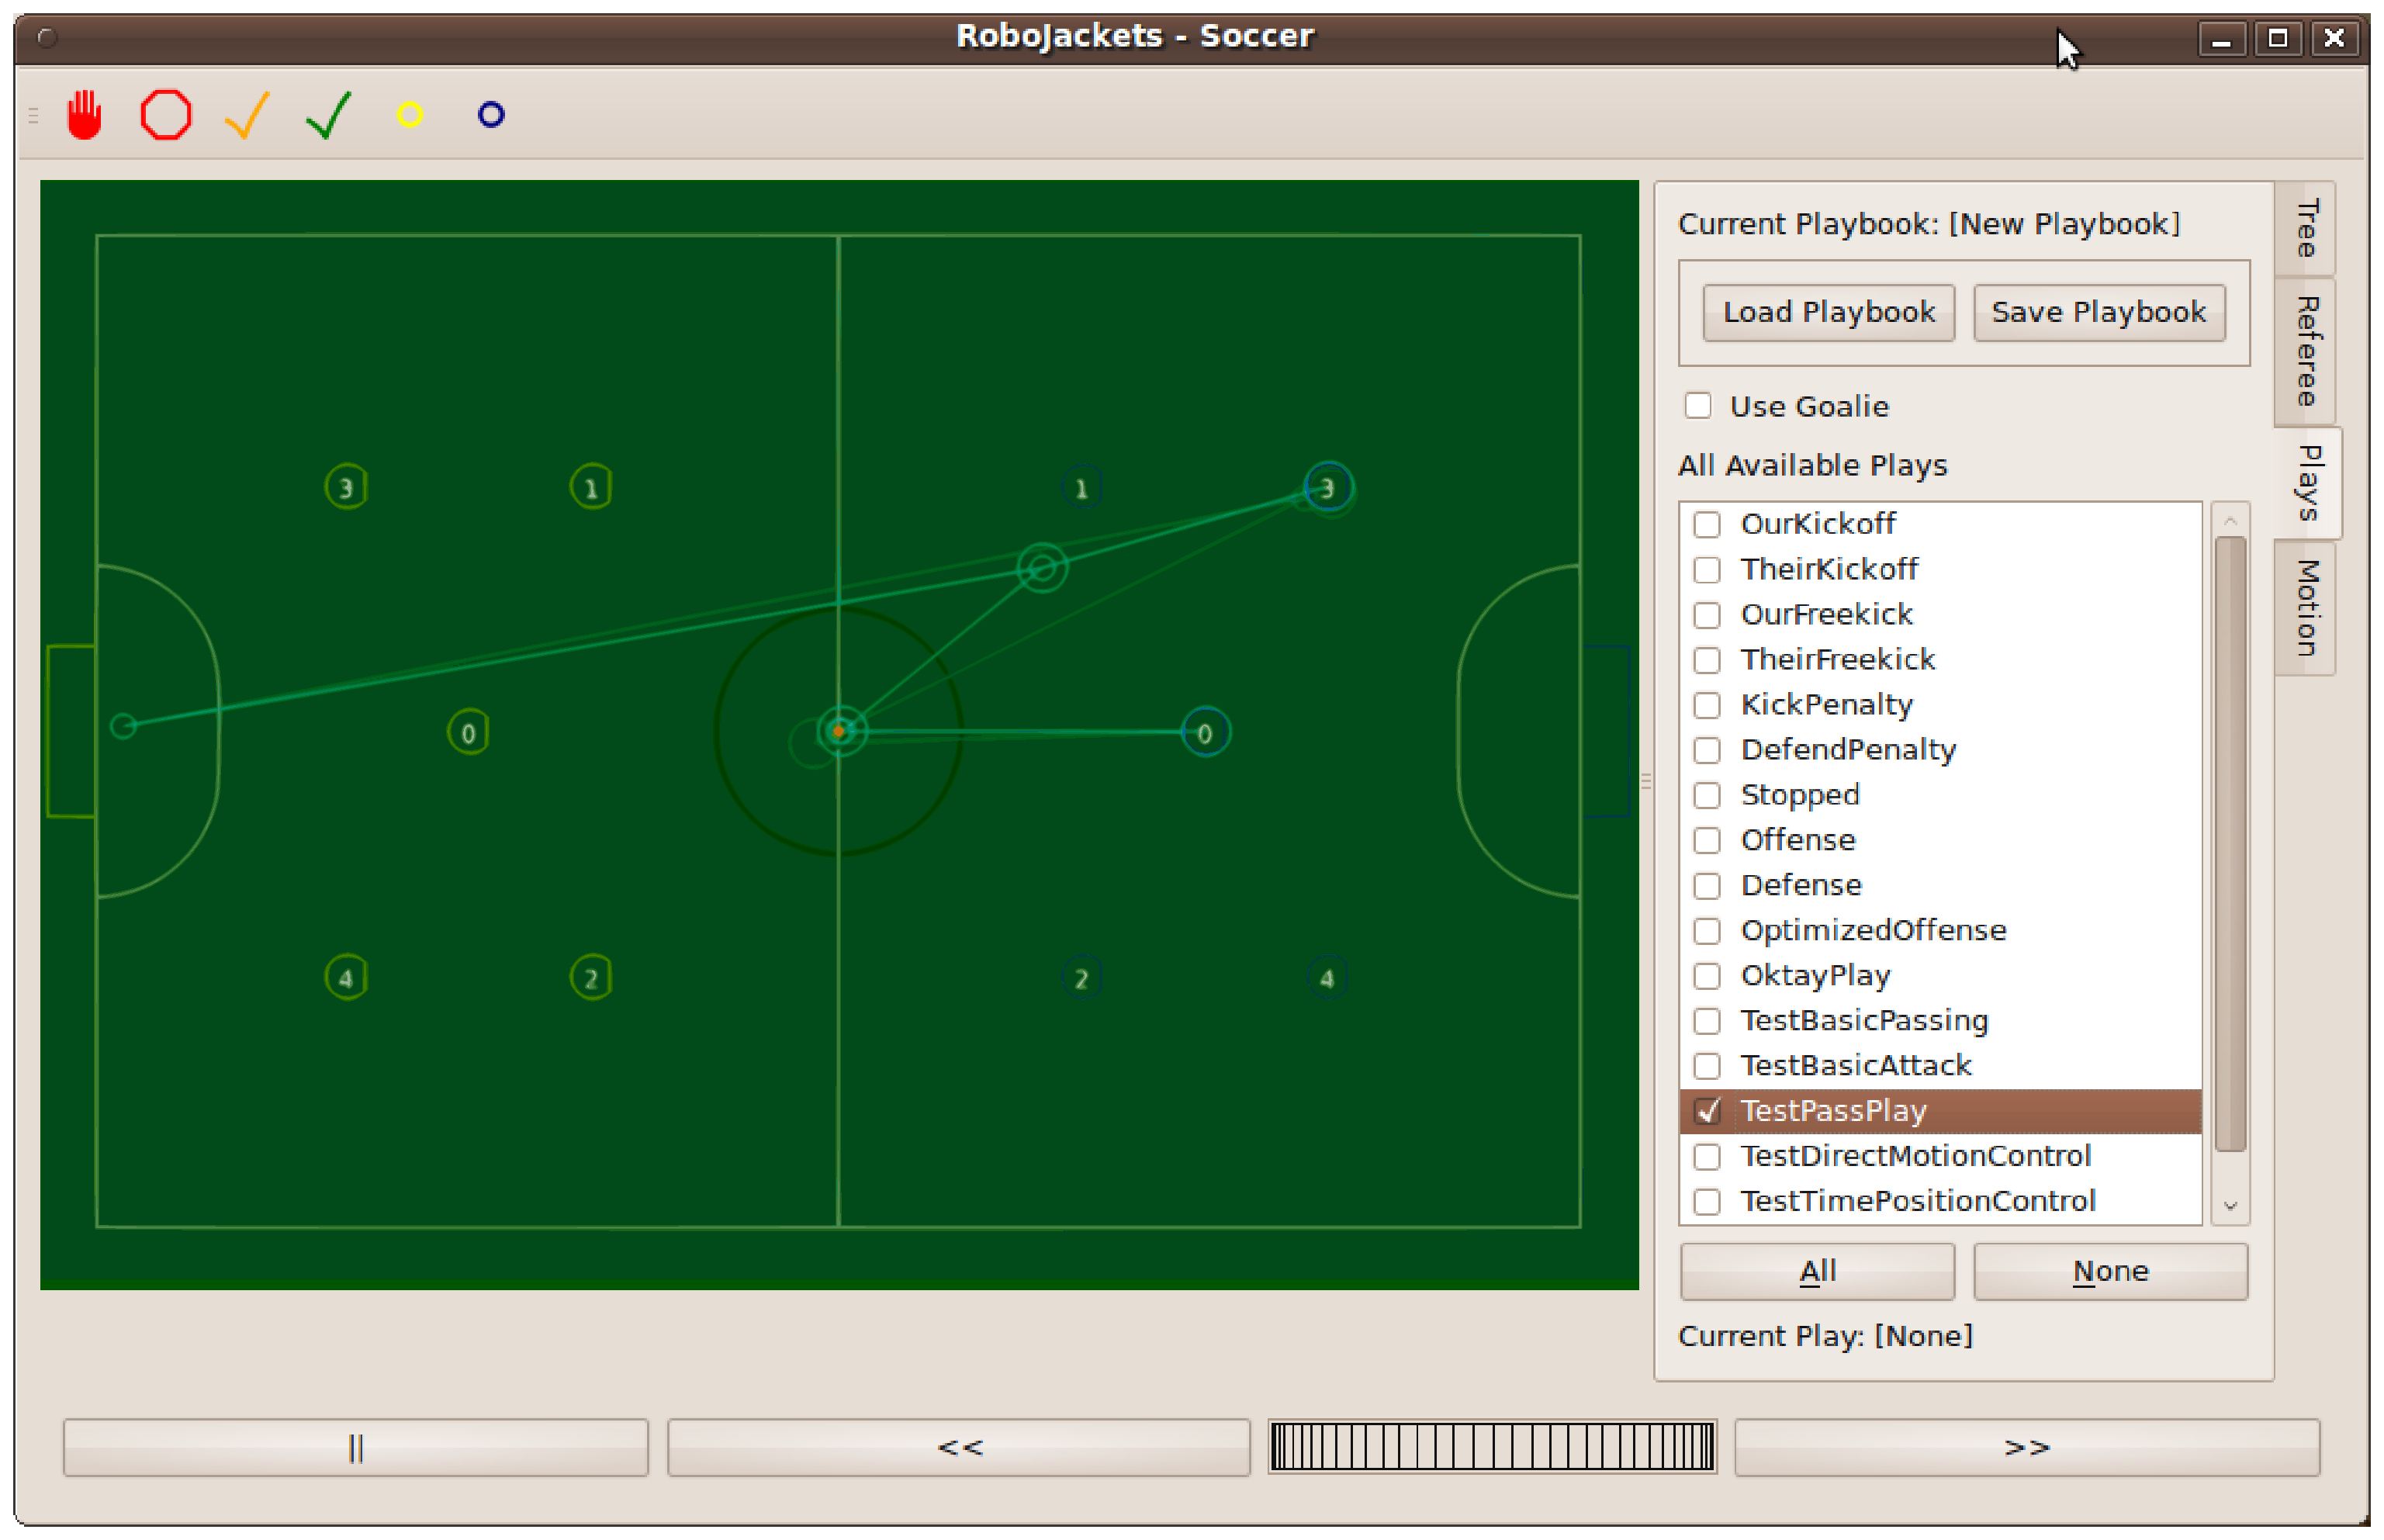
\includegraphics[totalheight=1.6in]{ui}
\end{center}
\caption{Simulator interface.}
\label{experiment1fig1}
\end{figure}


\begin{figure}[ht!]
\begin{center}
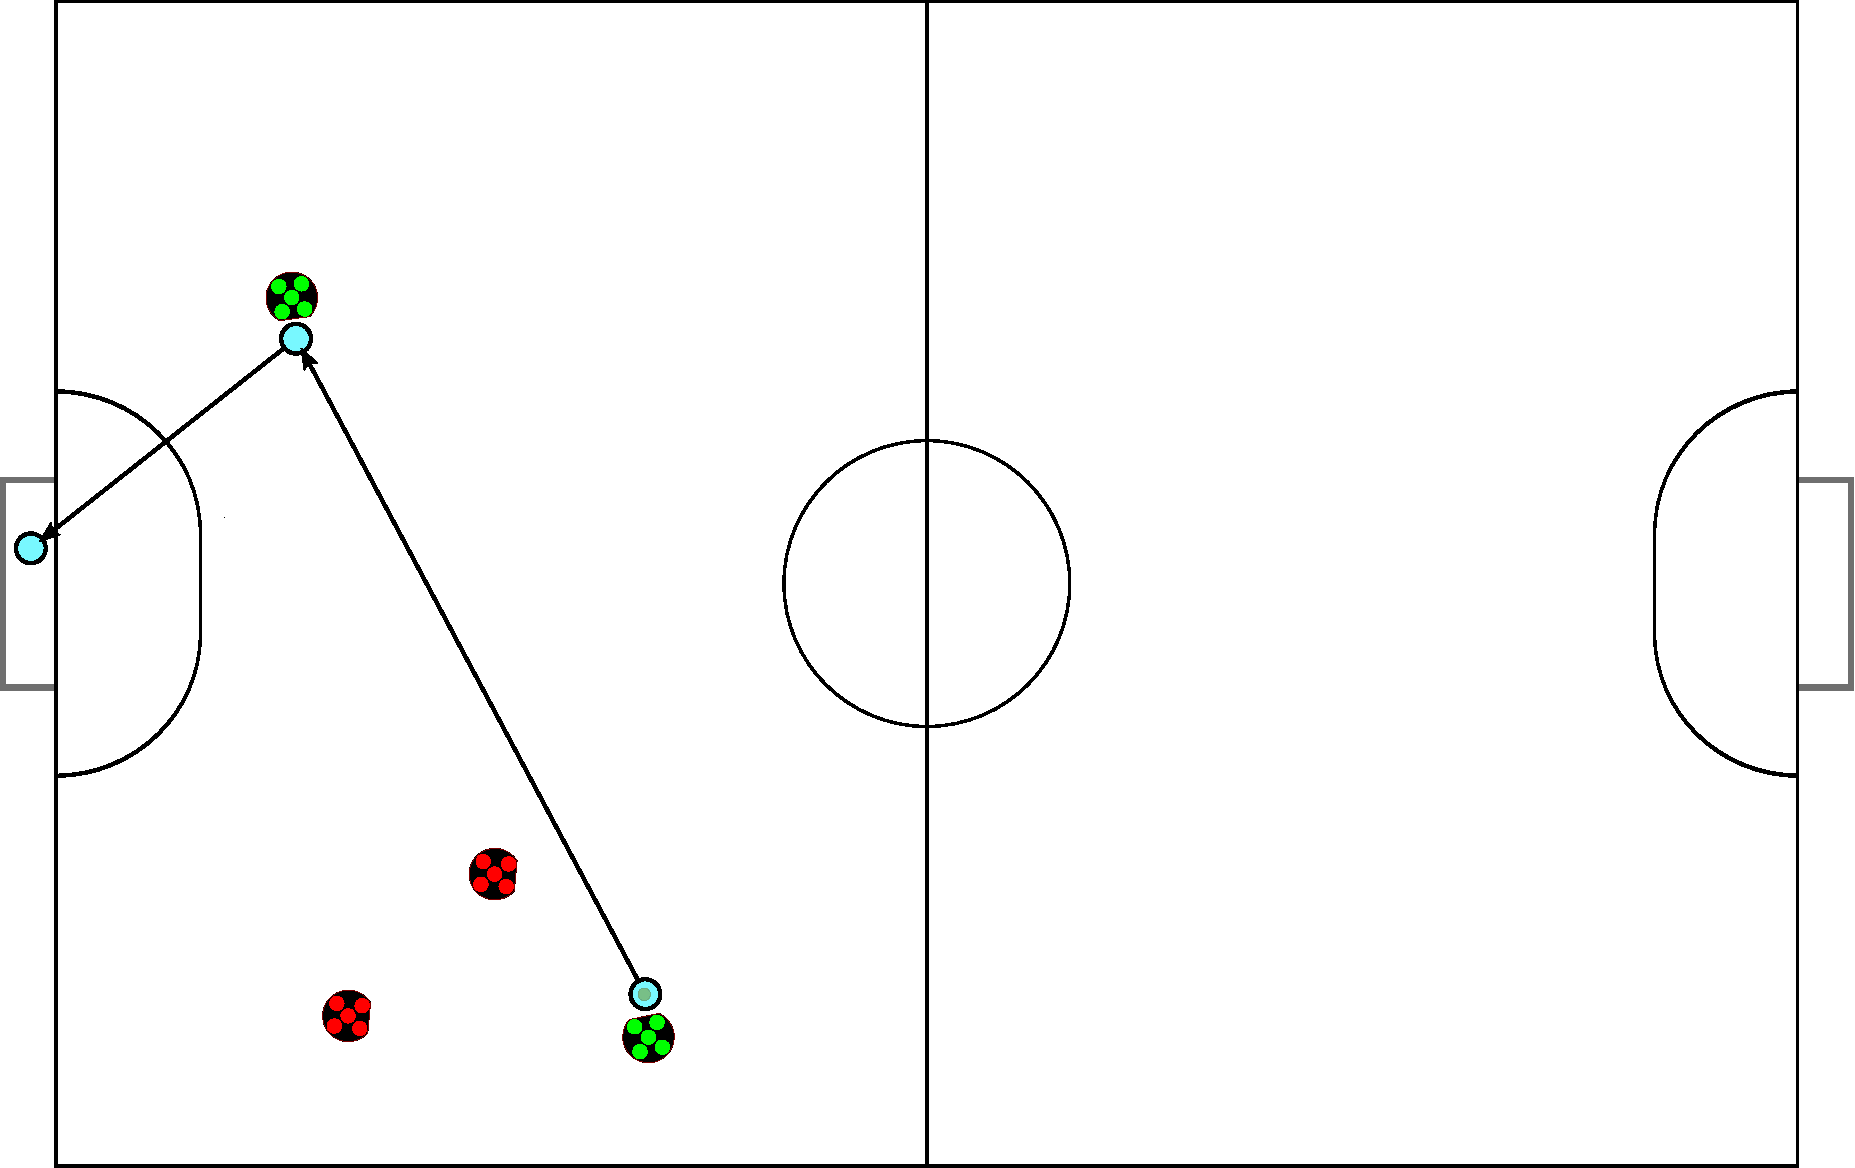
\includegraphics[totalheight=1.6in]{nonoptimized_plan}
\end{center}
\caption{Pass generated by the analytical solver, execution of the pass took 5 seconds. A videos of this experiment is available at http://tinyurl.com/regPass.}
\label{experiment1fig1}
\end{figure}

\begin{figure}[ht!]
\begin{center}
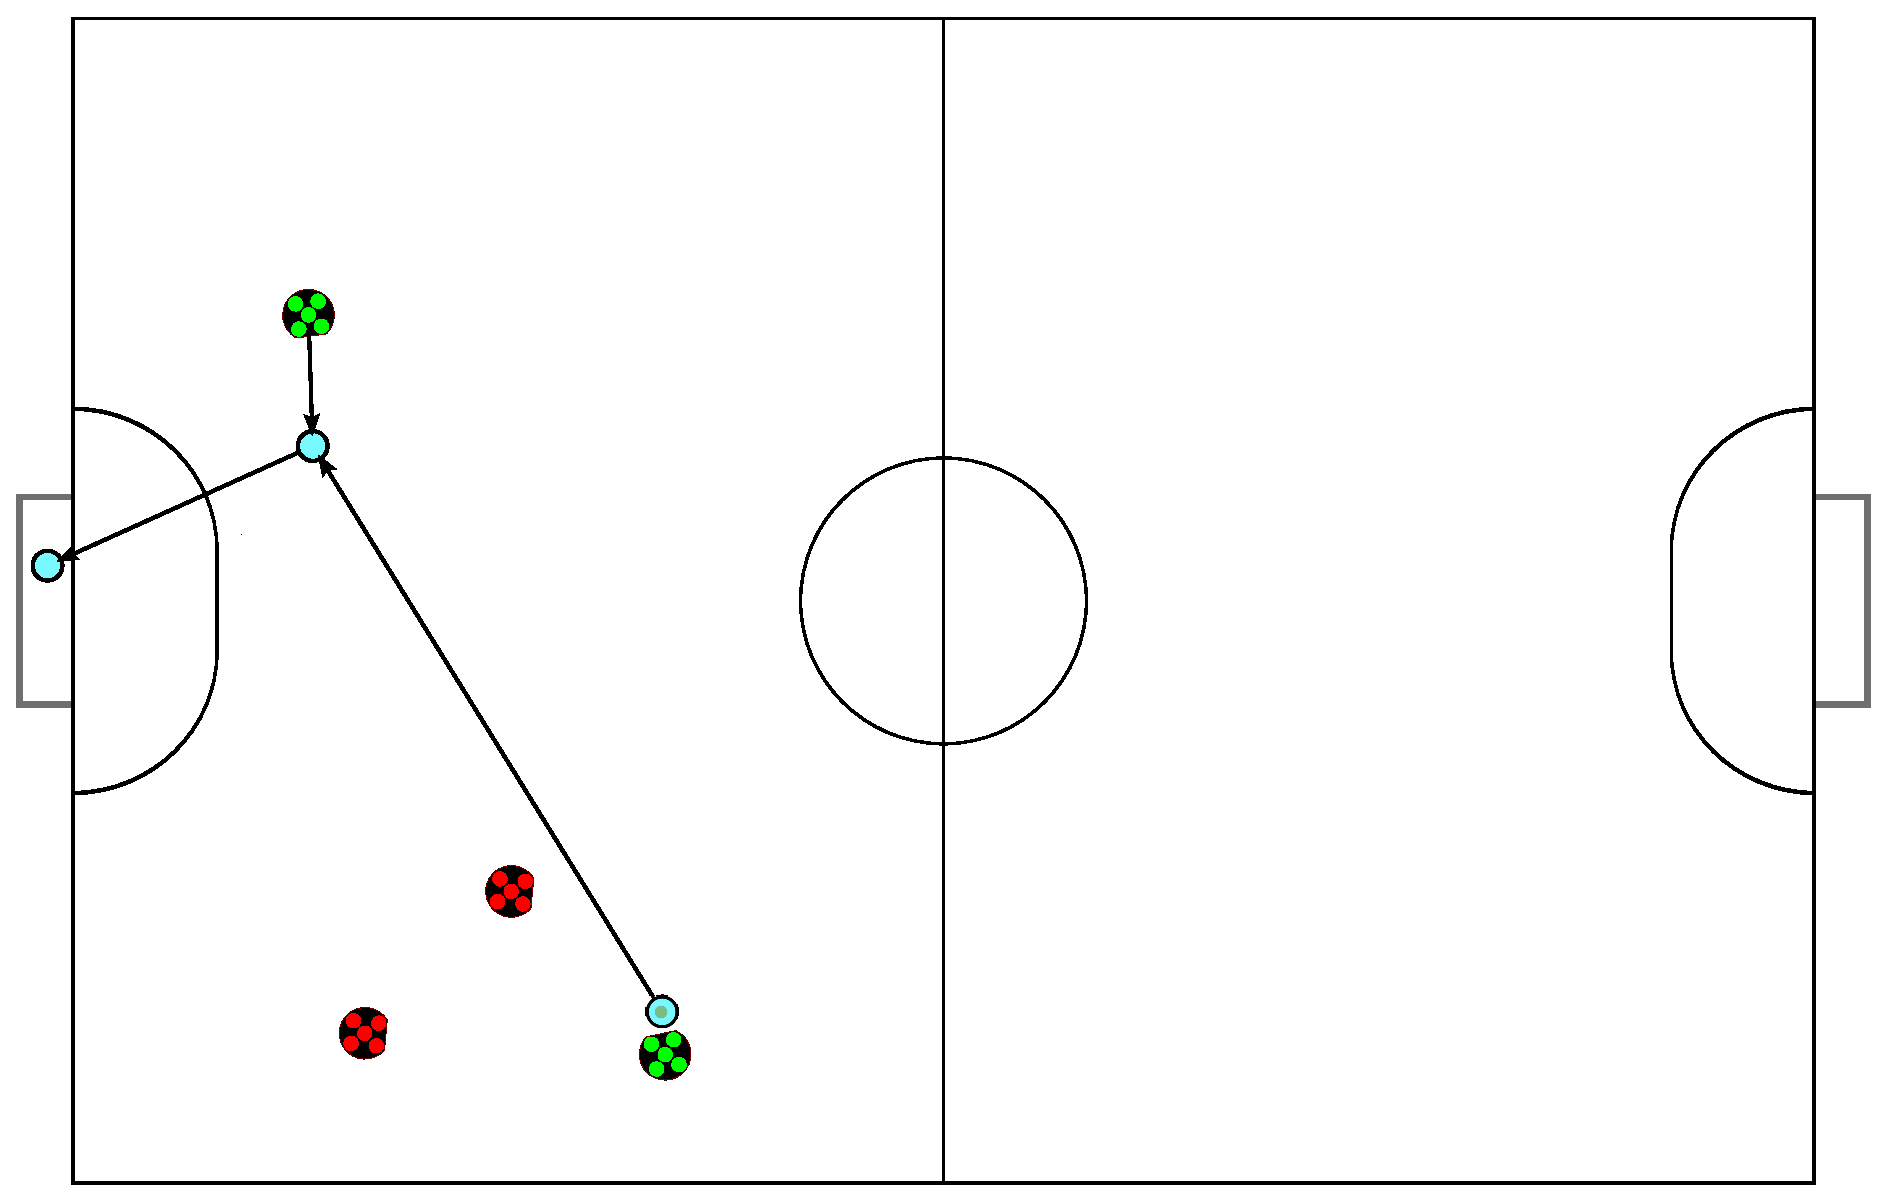
\includegraphics[totalheight=1.6in]{optimized_plan}
\end{center}
\caption{Pass after optimization, execution of the pass took 4 seconds. A videos of this experiment is available at http://tinyurl.com/optPass.}
\label{experiment1fig2}
\end{figure}

Our first type of experiments tested a non-optimized pass against an optimized pass under identical initial conditions, where the opponent team is static. As Fig. \ref{experiment1fig1} and Fig. \ref{experiment1fig2} show, the optimized pass is shorter, and the time required to execute the path is less as a result. We tested several variants of this experiment, and the optimizer consistently produced shorter paths. Additionally, the optimizer did not have a noticeable effect on performance.

Our second type of experiment tested both non-optimized and optimized passes in a dynamic scenario, where the opponent team consisted of one goalie and one defender from the 2008 GT Robocup team. Both of the passes were able to score on the previous team by using quick passes to get the ball past the goalie. The execution of the plans was not robust due to problems intercepting a fast-moving pass, which prevented consistent results comparing the optimized and non-optimized passes.

\section{ANALYSIS}
The results of the system, in a somewhat simplified form, indicate potential for this technique. Because our system uses much of the underlying code from our 2008 GT Robocup team to evaluate analytical solutions, our analytical solution step generalizes the ``0-pass'' direct goal kicks of our previous system to plans that include one or two additional robots. The optimization on top of this analytic solution was shown to improve the solutions by considering parameters that neither the 2008 GT Robocup team, nor the analytical solution were able to consider.
Our experiments have shown that our system can perform both high and low-level planning simultaneously, and while we were not able to test directly against a STP team, at a conceptual level our algorithm goes beyond the STP framework.

\section{DISCUSSION}
We learned a number of lessons from the development of this system, and there is a great deal that can be improved, but the combination of an analytic planner and an optimization engine appear to be an effective means of generating passing plans.  The optimizer has a great deal of flexibility, and even in a smaller example system, we have the flexibility to make the system very robust.  Further work could improve the system by integrating a motion model into the factor graph itself, and then bypassing the underlying RRT-based planner to make plans more predictable. 
\begin{itemize}
\item The multi-stage planner allows evaluation of plans we would not have been able to find otherwise
\item While the current optimization approach uses a simpler cost function, the system is very scalable
\item We need to improve the interactions between the low-level control and the planner outputs
\end{itemize}


%%%%%%%%%%%%%%%%%%%%%%%%%%%%%%%%%%%%%%%%%%%%%%%%%%%%%%%%%%%%%%%%%%%%%%%%%%%%%%%%

\section{ACKNOWLEDGMENTS}

The authors would like to thank the GT RoboCup SSL team for developing the system used for this project, and in particular Ben Johnson and the rest of the software team for managing many of the background details of keeping the entire robot control system functional. 


\bibliographystyle{unsrt}
\bibliography{RIPFinal}

\end{document}
